\section{Introduction}

In order to set limits and generate criteria for the realization of the project, the group decided to give the project an application, rather than just designing a control system for the P\&T setup. The following ideas were considered and graded.

\subsection{Object Balancing}
An object is placed on a plate attached to the P\&T system. The core of this project is the balancing of the object, making sure it remains still on the plate. It should also be possible to move the plate to make the object move to a specific location on the surface.
Expansion: Furthermore, a labyrinth could be designed for the P\&T system to navigate a ball through.

\subsection{Spotlight Control}
A spotlight is attached to the system, making it adjustable without physically moving the system. The P\&T system is used to point the spotlight to the desired position. This can be done by either giving the system coordinates or by creating an application that moves the spotlight through predefined patterns.

\subsection{Triangulation}
This would involve the triangulation of a signal, using the P\&T movement to point something in the direction of it. An example use for this could be a camera attached to the P\&T system, recording a person carrying a signaling device.

\subsection{Basis of Evaluation}
Choice of the project is based on the following criteria:

\begin{enumerate}
\item Difficulty
\begin{enumerate}
\item Is the project reasonable in respect to making early progress?
\item Is the project sufficiently complex?
\end{enumerate}
\item Interest - Does the project seem interesting? 
\item Curriculum relevance - To what degree does the project relate to the courses of the semester?
\item Practical relevance
\end{enumerate}

\begin{figure}[h!]
\centering
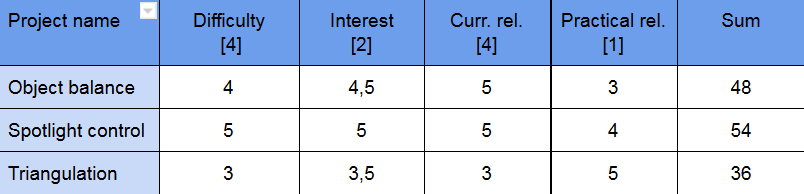
\includegraphics[scale=0.7]{Billeder/ProjectEvaluation.png}
\caption{Table evaluating the merit of different project ideas}
\label{fig:ProjectEvaluation}
\end{figure}

Through this evaluation, the spotlight control project was decided upon. From this point, every decision was made with respect to this selection.